% =====================================================================
%  MODELO DE TRABALHO / RELATÓRIO
%  Astronomia (AST0001) -- Curso de Física -- UDESC Joinville
%
%  COMO USAR:
%   1. Preencha os quatro campos logo abaixo (nome, título do trabalho).
%   2. Escreva o conteúdo nas seções marcadas.
%   3. Compile com pdfLaTeX duas vezes (a segunda resolve as referências).
%
%  Tudo que começa com % é comentário: o LaTeX ignora, e serve para
%  explicar o que cada comando faz. Leia os comentários -- eles são a
%  parte mais útil deste arquivo.
% =====================================================================

\documentclass[12pt,a4paper]{article}

% ---------------------------------------------------------------- pacotes
\usepackage[utf8]{inputenc}      % acentuação no arquivo fonte
\usepackage[T1]{fontenc}         % acentuação correta no PDF gerado
\usepackage[brazil]{babel}       % hifenização e nomes em português
\usepackage{lmodern}
\usepackage[margin=2.5cm]{geometry}
\usepackage{graphicx}            % incluir figuras
\usepackage{amsmath,amssymb}     % equações
\usepackage{booktabs}            % tabelas com traços de qualidade
\usepackage{siunitx}             % unidades físicas bem formatadas
\usepackage{float}               % opção [H] para fixar figuras
\usepackage{caption}
\usepackage[colorlinks=true,linkcolor=blue,urlcolor=blue]{hyperref}

\sisetup{output-decimal-marker={,}, input-decimal-markers={.,}, per-mode=symbol}  % vírgula decimal

% ---------------------------------------------------- PREENCHA AQUI
\newcommand{\aluno}{Nome Completo do Aluno}
\newcommand{\titulotrabalho}{Título do Trabalho}
\newcommand{\disciplina}{ASTRONOMIA (AST0001)}
\newcommand{\semestre}{2026/2}
% -------------------------------------------------------------------

\begin{document}

% =====================================================================
%  CAPA
% =====================================================================
\begin{titlepage}
\centering


\includegraphics[width=0.30\textwidth]{udesc.png}\par
\vspace{0.8cm}

{\large UNIVERSIDADE DO ESTADO DE SANTA CATARINA\par}
{\large Centro de Ciências Tecnológicas --- CCT\par}
{\large Curso de Física\par}

\vspace{2.5cm}

{\Large \disciplina\par}

\vspace{1.5cm}

\rule{\textwidth}{0.4pt}\par
\vspace{0.6cm}
{\huge\bfseries \titulotrabalho\par}
\vspace{0.6cm}
\rule{\textwidth}{0.4pt}\par

\vspace{2.5cm}

{\Large \aluno\par}

\vfill

{\large Joinville --- SC\par}
{\large \semestre\par}

\end{titlepage}

% Sumário: útil em trabalhos longos. Apague as duas linhas se não quiser.
\tableofcontents
\newpage

% =====================================================================
\section{Introdução}
% =====================================================================
% O QUE ESCREVER AQUI:
%  - de que assunto trata o trabalho e por que ele importa;
%  - qual pergunta você quer responder;
%  - se for um relatório de experimento ou laboratório, descreva o que
%    foi feito, com que dados e em que condições;
%  - o que o leitor vai encontrar nas seções seguintes.
% Escreva em 2 ou 3 parágrafos. Não copie texto de fonte alguma.

Escreva aqui a apresentação do assunto. Explique o contexto físico, diga
qual pergunta o trabalho responde e descreva brevemente a experiência ou
o conjunto de dados utilizado.

No último parágrafo, anuncie a organização do texto. Por exemplo: a
Seção~\ref{sec:teoria} apresenta as equações usadas, a
Seção~\ref{sec:dados} traz os dados e os resultados, e a
Seção~\ref{sec:conclusao} discute o que foi obtido.

% =====================================================================
\section{Teoria Básica}
\label{sec:teoria}
% =====================================================================
% O QUE ESCREVER AQUI:
%  - as equações que você vai efetivamente usar, e nada além disso;
%  - o significado de cada símbolo;
%  - as hipóteses que cada equação assume.
% Regra prática: toda equação que aparece aqui precisa ser usada na
% Seção de Dados. Equação que não é usada não entra.

Apresente aqui as relações físicas empregadas. Cada símbolo deve ser
definido, e cada hipótese, declarada.

% --- EXEMPLO 1: equação numerada, para ser citada depois -------------
A energia recebida por unidade de área e tempo cai com o quadrado da
distância:
\begin{equation}
    F = \frac{L}{4\pi d^{2}},
    \label{eq:inverso-quadrado}
\end{equation}
em que $F$ é o fluxo, $L$ a luminosidade da fonte e $d$ a distância. A
Equação~\eqref{eq:inverso-quadrado} supõe emissão isotrópica e ausência
de absorção no caminho.

% --- EXEMPLO 2: como citar uma equação no meio do texto --------------
Note que a Equação~\eqref{eq:inverso-quadrado} é a base do módulo de
distância. Para citar uma equação, use \verb|\eqref{rótulo}|; o número é
atualizado sozinho se você inserir outra equação antes dela.

% --- EXEMPLO 3: várias linhas alinhadas ------------------------------
Quando há uma sequência de passos, use o ambiente \texttt{align} e
alinhe pelo sinal de igual:
\begin{align}
    m - M &= -2{,}5\log_{10}\left(\frac{F(d)}{F(10\,\mathrm{pc})}\right)
           = -2{,}5\log_{10}\left(\frac{10\,\mathrm{pc}}{d}\right)^{2} \nonumber\\
          &= 5\log_{10}\left(\frac{d}{\mathrm{pc}}\right) - 5.
    \label{eq:modulo}
\end{align}

% --- EXEMPLO 4: equação sem número -----------------------------------
Se a equação for auxiliar e você não pretende citá-la, use o ambiente
com asterisco, que não gera numeração:
\begin{equation*}
    d\,[\mathrm{pc}] = \frac{1000}{p\,[\mathrm{mas}]}.
\end{equation*}

% --- EXEMPLO 5: matemática dentro do texto e unidades ----------------
Símbolos no meio da frase vão entre cifrões: a paralaxe de Proxima
Centauri vale $p = \SI{768}{mas}$, o que corresponde a
$d = \SI{1,30}{pc}$. Para números com unidade, o comando
\verb|\SI{valor}{unidade}| cuida do espaçamento e da formatação, e
escreve $\SI{3,0e8}{\meter\per\second}$ corretamente.

% =====================================================================
\section{Dados}
\label{sec:dados}
% =====================================================================
% O QUE ESCREVER AQUI:
%  - de onde vieram os dados (arquivo, laboratório, catálogo);
%  - a tabela com os valores medidos e os calculados;
%  - as figuras;
%  - o resultado numérico principal, COM incerteza e COM unidade.
% Toda tabela e toda figura precisam ser citadas no texto. Uma figura
% que ninguém menciona não deveria estar no trabalho.

Descreva a origem dos dados e apresente os resultados. Diga quantas
medidas foram usadas e que critério de seleção foi aplicado.

% --- EXEMPLO 6: tabela ----------------------------------------------
% Estrutura: \begin{table} -> \caption -> \begin{tabular} -> dados.
% O argumento {lccc} diz o alinhamento de cada coluna:
%   l = esquerda, c = centro, r = direita.
% O & separa colunas e o \\ termina a linha.
A Tabela~\ref{tab:exemplo} mostra o formato recomendado: uma linha por
objeto, uma coluna por grandeza, unidades no cabeçalho e incertezas
junto do valor.

\begin{table}[H]
    \centering
    \caption{Paralaxe, distância e magnitude absoluta de quatro estrelas
             próximas. As distâncias vêm de $d = 1/p$ e as magnitudes
             absolutas da Equação~\eqref{eq:modulo}.}
    \label{tab:exemplo}
    \begin{tabular}{lcccc}
        \toprule
        Estrela & $p$ (mas) & $d$ (pc) & $G$ (mag) & $M_G$ (mag) \\
        \midrule
        Proxima Centauri & $768{,}07 \pm 0{,}05$ & $1{,}302$ & $8{,}98$ & $15{,}5$ \\
        Estrela de Barnard & $546{,}98 \pm 0{,}04$ & $1{,}828$ & $8{,}19$ & $13{,}9$ \\
        Wolf 359 & $415{,}18 \pm 0{,}07$ & $2{,}409$ & $11{,}04$ & $16{,}1$ \\
        Lalande 21185 & $392{,}75 \pm 0{,}03$ & $2{,}546$ & $6{,}55$ & $11{,}5$ \\
        \bottomrule
    \end{tabular}
\end{table}

% --- EXEMPLO 7: figura ----------------------------------------------
% width=0.75\linewidth faz a figura ocupar 75% da largura do texto.
% O [H] exige que a figura fique exatamente aqui; sem ele, o LaTeX
% escolhe a melhor posição sozinho (o que costuma ser melhor).
A Figura~\ref{fig:exemplo} mostra o diagrama cor-magnitude construído a
partir das \num{2000} estrelas do catálogo. A sequência principal
aparece como a faixa diagonal, e o grupo isolado no canto inferior
esquerdo corresponde às anãs brancas.

\begin{figure}[H]
    \centering
    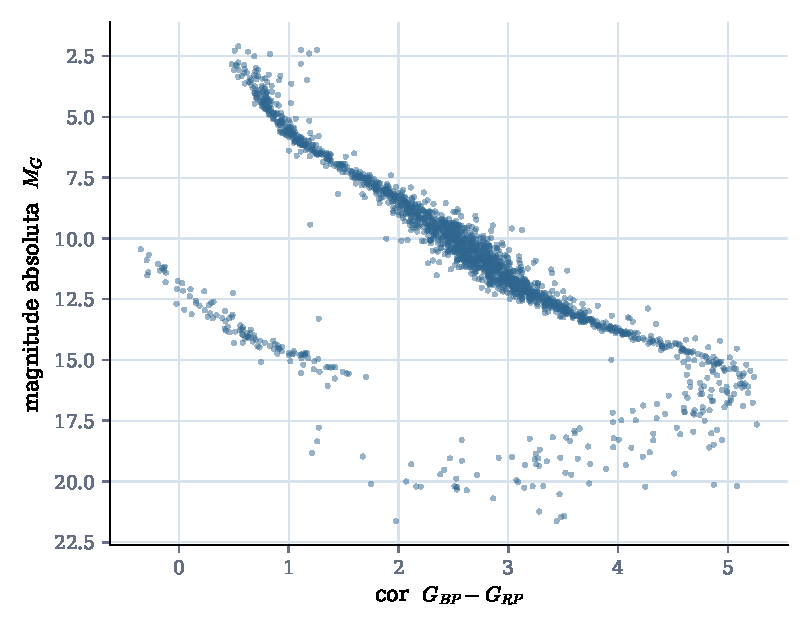
\includegraphics[width=0.75\linewidth]{figura_exemplo.pdf}
    \caption{Diagrama cor-magnitude de estrelas a menos de
             \SI{25}{pc} do Sol, com dados da missão Gaia. Cada ponto é
             uma estrela; o eixo vertical está invertido para que as
             mais luminosas apareçam em cima.}
    \label{fig:exemplo}
\end{figure}

% --- EXEMPLO 8: como apresentar um resultado -------------------------
% Um resultado numérico tem três partes obrigatórias: valor, incerteza
% e unidade. Sem as três, ele não é um resultado.
O valor obtido para a grandeza de interesse foi
\begin{equation*}
    H_0 = 69 \pm 3\ \mathrm{km\,s^{-1}\,Mpc^{-1}},
\end{equation*}
em que a incerteza citada é apenas estatística. Discuta separadamente as
fontes sistemáticas, se houver.

% =====================================================================
\section{Conclusão}
\label{sec:conclusao}
% =====================================================================
% O QUE ESCREVER AQUI:
%  - o que os números obtidos significam fisicamente;
%  - comparação com o valor esperado ou de referência, quando existir;
%  - a maior fonte de incerteza, e se ela é estatística ou sistemática;
%  - o que você mudaria para melhorar a medida.
% NÃO repita a introdução, e não introduza resultado novo aqui.

Discuta os resultados. Compare o valor obtido com o esperado e diga se a
diferença é compatível com as incertezas: uma discrepância de
$2\sigma$ pede explicação, uma de $0{,}5\sigma$ não.

Identifique a etapa que domina a incerteza final. Costuma ser mais
informativo dizer ``a incerteza vem da calibração de distância, não da
fotometria'' do que apresentar uma lista genérica de fontes de erro.

Termine dizendo o que uma medida melhor exigiria: mais dados, outro
instrumento, ou uma hipótese diferente no modelo.

% =====================================================================
% REFERÊNCIAS
% =====================================================================
% Liste apenas o que você realmente consultou. Para citar no texto, use
% \cite{rótulo} -- por exemplo: segundo Carroll e Ostlie \cite{carroll}.
\begin{thebibliography}{9}

\bibitem{carroll}
CARROLL, B. W.; OSTLIE, D. A.
\textit{An Introduction to Modern Astrophysics}. 2. ed.
Cambridge: Cambridge University Press, 2017.

\bibitem{apostila}
LIMA, R. C. R. de.
\textit{Astrofísica Moderna: capítulos de estudo}. UDESC, 2026.
Disponível em:
\url{https://rafaelcrdelima.github.io/Astronomia/}.

\bibitem{gaia}
GAIA COLLABORATION.
\textit{Gaia Data Release 3}. Arquivo público do ESA Gaia, 2022.
Disponível em: \url{https://gea.esac.esa.int/archive/}.

\end{thebibliography}

\end{document}
